\chapter{Aperçu conceptuel et Conception détaillée}
\label{chap:conception}

\section*{Introduction}
\addcontentsline{toc}{section}{Introduction}

La phase de conception est une étape très importante dans le cycle de développement de notre CRM intelligent. Tout d’abord, nous devons clarifier la vision globale de l’architecture. Ensuite, nous devons décrire en détail la conception de chaque module. Cette description comprend les vues statiques, qui sont présentées via le diagramme de classes d’entités, et les vues dynamiques, qui détaillent le fonctionnement interne de l’application à travers les diagrammes de séquences de conception et les diagrammes de classes participantes. L’objectif principal de la phase de conception est de transformer les spécifications établies dans le chapitre précédent en modèles techniques clairs. Cela prépare le terrain pour la phase de réalisation de notre CRM intelligent.

%──────────────────────────────────────────────────────
\section{Architecture physique et logique}
%──────────────────────────────────────────────────────

\subsection{Architecture 3-tiers orientée services}

Nous avons choisi, pour la conception de notre solution CRM Micro-SaaS, une architecture basée sur le modèle à 3 niveaux, complétée par une approche de micro-services pour intégrer l’intelligence artificielle. Ce modèle logique a pour but de dissocier clairement les responsabilités au sein du système. Cette architecture comporte trois niveaux que l'on peut décrire brièvement comme suit :
\begin{itemize}
    \item \textbf{Couche présentation (Frontend) :} Il s'agit de la partie de l'application que l'utilisateur voit et avec laquelle il interagit. Elle est développée avec \textbf{Next.js} et React, et offre une interface dynamique, réactive et sécurisée.
    \item \textbf{Couche applicative (Backend et Services IA) :} C’est le cerveau de l’application. Elle contient la logique métier et les règles de gestion, et traite toutes les requêtes des utilisateurs. Cette couche est constituée de deux éléments principaux : le serveur principal en \textbf{NestJS} qui gère les entités du CRM, et un micro-service en \textbf{FastAPI} dédié exclusivement au \textit{lead scoring} par intelligence artificielle.
    \item \textbf{Couche d’accès aux données :} C’est la couche responsable de la persistance des données. Elle utilise le système de gestion de bases de données relationnelles \textbf{MySQL} et l’ORM \textbf{Prisma} pour garantir la sécurité et la cohérence des données lors des opérations de lecture et d’écriture.
\end{itemize}

\begin{figure}[H]
    \centering
     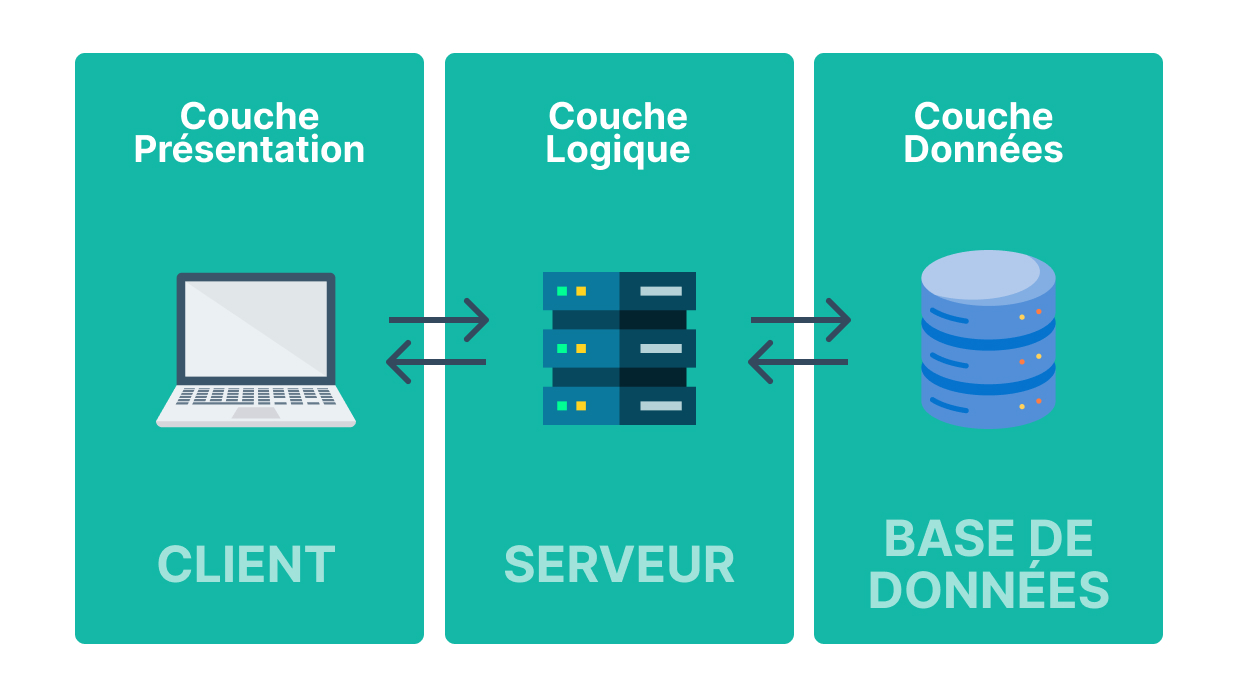
\includegraphics[width=\textwidth,height=0.82\textheight,keepaspectratio]{images/architecture_3tiers.png}
    \caption{Architecture globale de l'application (Image manquante)}
    \label{fig:architecture_globale}
\end{figure}

%──────────────────────────────────────────────────────
\section{Patrons de conception}
%──────────────────────────────────────────────────────

Lors du développement d'applications complexes comme un CRM, nous faisons souvent face à certains problèmes de conception récurrents. Pour les résoudre de manière efficace et réutilisable, nous utilisons des patrons de conception (\textit{Design Patterns}). Ce sont des modèles reconnus permettant non seulement de résoudre un problème, mais aussi d’améliorer la qualité du code, sa maintenabilité et d’accélérer le processus de développement.

\subsection{Patron de conception MVC (Modèle-Vue-Contrôleur)}

Le \textit{Model-View-Controller} (MVC) est l’un des patrons de conception les plus utilisés pour le développement web. Bien que physiquement réparti entre le frontend et le backend dans notre système moderne, son principe conceptuel régit notre application :
\begin{itemize}
    \item \textbf{Modèle :} Géré par Prisma et NestJS, il représente les données pures de l’application (Leads, Contacts, Deals, etc.) et encapsule la logique de manipulation des données.
    \item \textbf{Vue :} Gérée par Next.js à travers des composants React (TailwindCSS, Shadcn UI), elle permet de présenter et de mettre en forme les données du modèle pour l’utilisateur final de façon réactive.
    \item \textbf{Contrôleur :} Implémenté via les contrôleurs NestJS et les Server Actions de Next.js, il se place entre la vue et le modèle. Il intercepte les requêtes de l'utilisateur, sollicite les services adéquats et retourne la réponse formatée.
\end{itemize}

\begin{figure}[H]
    \centering
     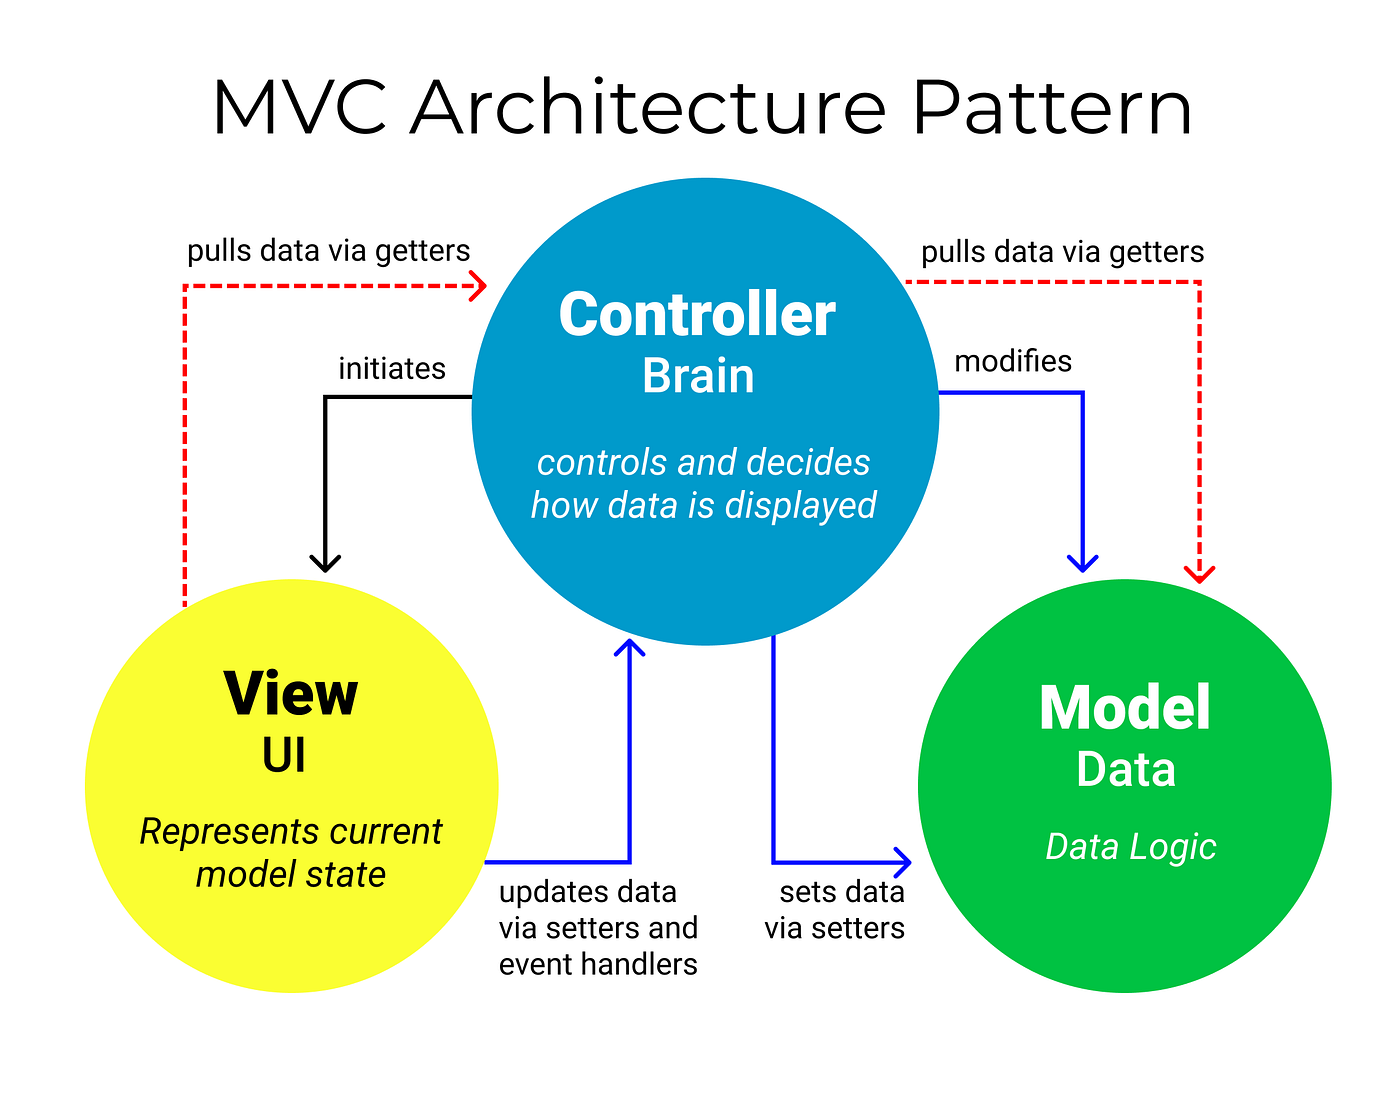
\includegraphics[width=0.95\textwidth,height=0.78\textheight,keepaspectratio]{images/patron_mvc.png}
    \caption{Principe du patron de conception MVC dans l'application (Image manquante)}
    \label{fig:patron_mvc}
\end{figure}

\subsection{Patron de conception DAO (Data Access Object) / Repository}

Le patron de conception DAO permet de séparer la logique métier de la logique d’accès aux données. Dans notre projet, le rôle de DAO est assuré de manière moderne par \textbf{Prisma Client}. 

Les objets de données sont représentés par des modèles (schémas Prisma), qui sont généralement simples et ne contiennent que les informations de la base. Les services NestJS utilisent les méthodes fournies par l'ORM pour effectuer les opérations CRUD sans écrire de requêtes SQL brutes, assurant ainsi une abstraction sécurisée de la source de données.

\begin{figure}[H]
    \centering
    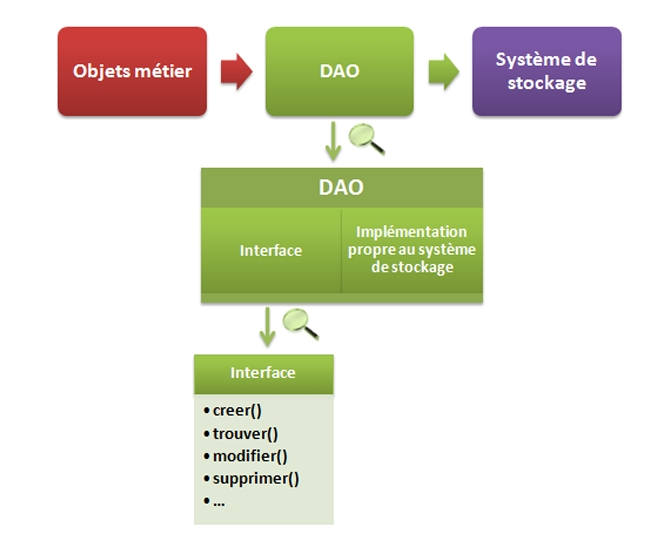
\includegraphics[width=0.95\textwidth,height=0.78\textheight,keepaspectratio]{images/patron_dao.png}
    \caption{Principe du patron de conception DAO avec Prisma (Image manquante)}
    \label{fig:patron_dao}
\end{figure}

\subsection{Patron de conception DTO (Data Transfer Object)}

Le patron de conception DTO est un modèle qui permet de séparer la logique métier de l’application de la logique de transfert de données. Le principe de ce patron est de créer une classe qui contient les données que l’on souhaite transférer, sans comportement métier associé.

Dans notre architecture NestJS, les DTOs sont utilisés pour encapsuler les données et les transférer entre le client et le backend. Décorés avec \textit{class-validator}, ils garantissent que seules les données valides, typées et autorisées transitent sur le réseau, sécurisant ainsi les endpoints de l'API.

\begin{figure}[H]
    \centering
    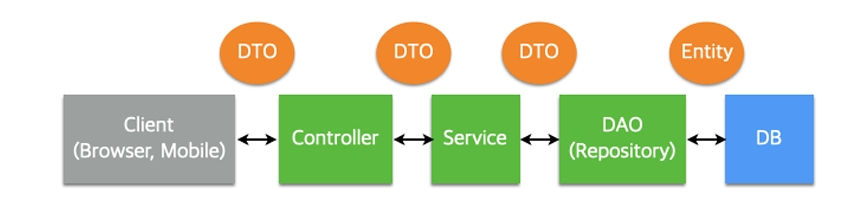
\includegraphics[width=0.95\textwidth,height=0.78\textheight,keepaspectratio]{images/patron_dto.png}
    \caption{Principe du patron de conception DTO}
    \label{fig:patron_dto}
\end{figure}

%──────────────────────────────────────────────────────
\section{Conception détaillée}
%──────────────────────────────────────────────────────

Afin d’avoir une vue claire et approfondie sur la structure interne du système, nous allons présenter en premier lieu le diagramme de classes des entités de la solution entière. Ensuite, nous exposerons la conception détaillée des modules principaux à l’aide des diagrammes de classes participantes et des diagrammes de séquences de conception.

\subsection{Diagramme de classe d’entités}

Ce diagramme est souvent considéré comme le diagramme le plus important dans la modélisation orientée-objet. Il s’agit d’une représentation statique des éléments constituant un système avec leurs attributs et leurs opérations ainsi que les différentes relations entre eux.

Le modèle conceptuel de données de notre CRM gravite autour d'entités centrales structurant l'activité commerciale : \texttt{User}, \texttt{Company}, \texttt{Contact}, \texttt{Lead}, \texttt{Deal}, \texttt{Task} et \texttt{Ticket}.

\begin{figure}[H]
    \centering
    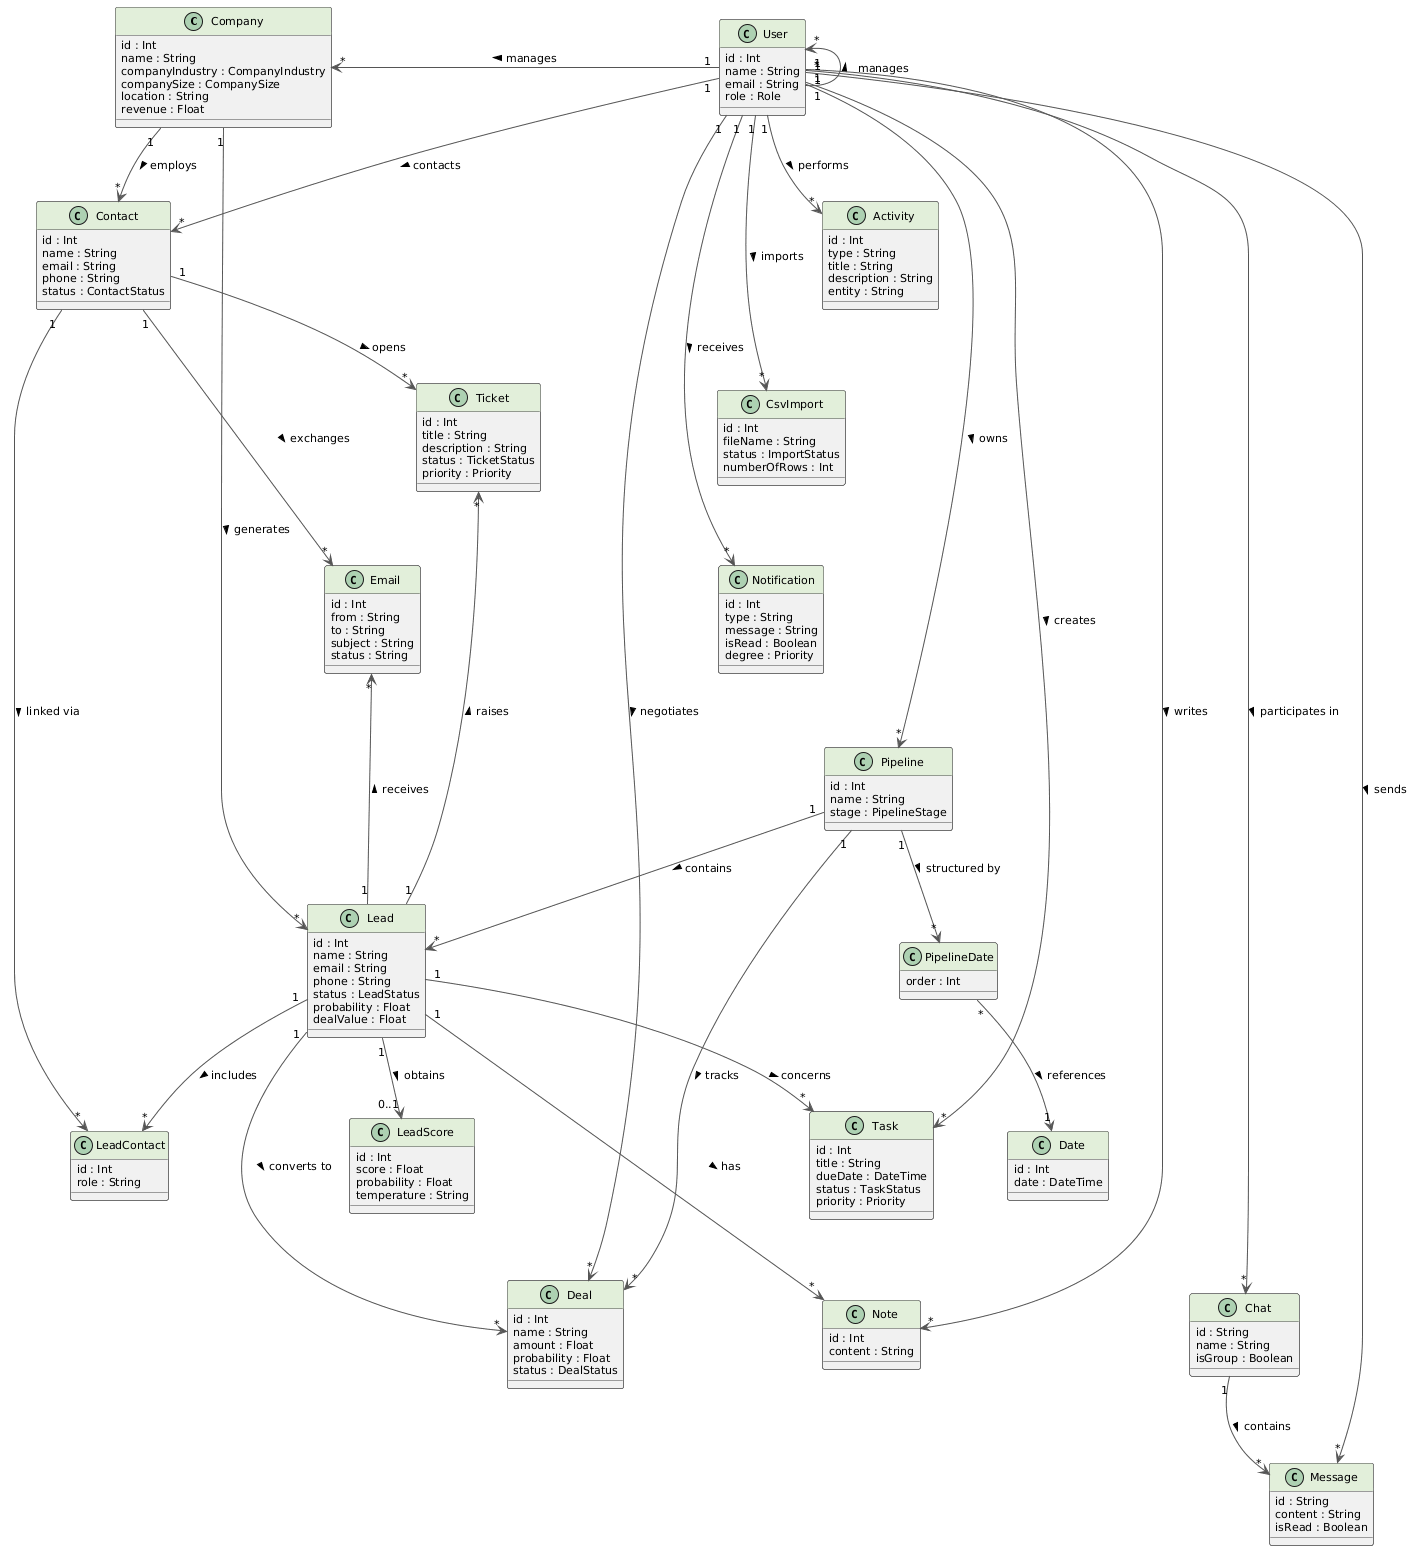
\includegraphics[width=\textwidth,height=0.86\textheight,keepaspectratio]{images/diagramme_classes_entites.png}
    \caption{Diagramme de classe d'entités du CRM}
    \label{fig:diagramme_classes}
\end{figure}

\begin{figure}[H]
    \centering
    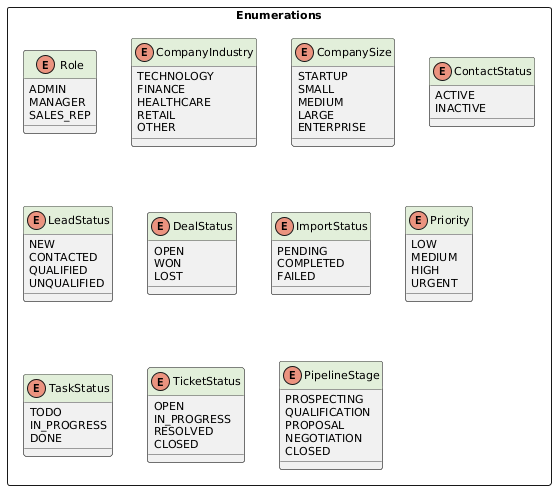
\includegraphics[width=\textwidth,height=0.82\textheight,keepaspectratio]{images/diagramme_classes_enumerations.png}
    \caption{Énumérations utilisées dans le modèle de données}
    \label{fig:diagramme_enumerations}
\end{figure}

\subsection{Diagrammes de séquences de conception (DSC)}

Les diagrammes de séquences permettent de modéliser comment les éléments internes du système interagissent entre eux selon un point de vue chronologique, en dévoilant l'appel des méthodes entre les contrôleurs, les services, et la base de données.

\subsubsection{Diagramme de séquence de conception \og~S'authentifier~\fg{}}

Lorsqu'un utilisateur tente de se connecter, le contrôleur d'authentification (\texttt{AuthController}) réceptionne la requête. Il fait appel au \texttt{AuthService} qui, à son tour, vérifie l'existence du compte via le \texttt{UsersService} et valide le hachage du mot de passe. Si le mot de passe correspond, un jeton d'accès JWT est généré et retourné pour être stocké dans le navigateur.

\begin{figure}[H]
    \centering
    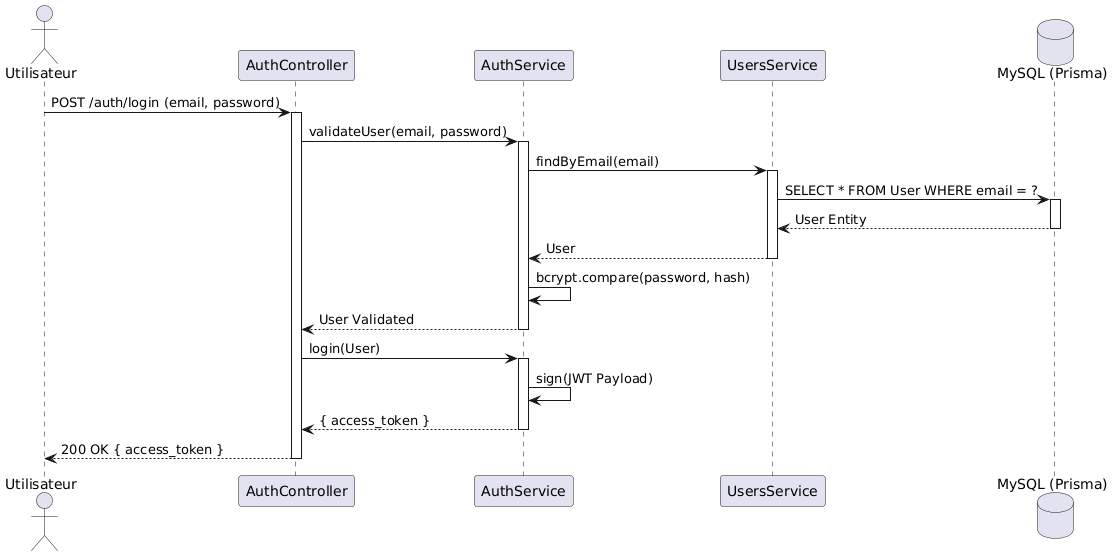
\includegraphics[width=\textwidth,height=0.82\textheight,keepaspectratio]{images/dsc_authentification.png}
    \caption{Diagramme de séquence de conception \og~S'authentifier~\fg{}}
    \label{fig:dsc_auth}
\end{figure}

\subsubsection{Diagramme de séquence de conception \og~Calculer Score IA (Lead Scoring)~\fg{}}

Pour évaluer la probabilité de conversion d'un prospect, le système interagit avec le micro-service IA. Le \texttt{LeadsController} invoque le \texttt{LeadsService}, qui assemble les données pertinentes du lead. Ces données sont expédiées par requête HTTP POST au \texttt{FastAPI AI Agent}. L'agent retourne un score calculé par son modèle d'apprentissage automatique. Le \texttt{LeadsService} met alors à jour l'entité \texttt{Lead} via Prisma et retourne le résultat complet.

\begin{figure}[H]
    \centering
    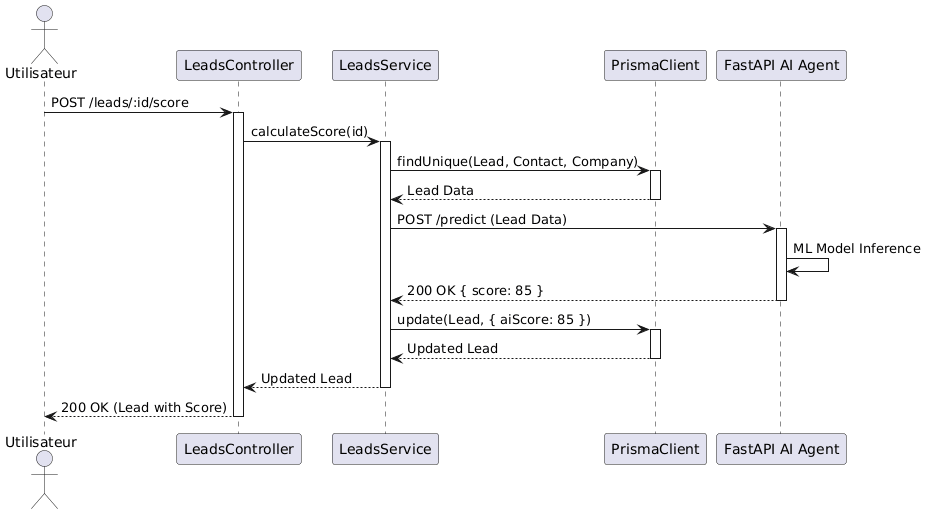
\includegraphics[width=\textwidth,height=0.82\textheight,keepaspectratio]{images/dsc_scoring_ia.png}
    \caption{Diagramme de séquence de conception \og~Calculer Score IA~\fg{}}
    \label{fig:dsc_scoring}
\end{figure}

\subsubsection{Diagramme de séquence de conception \og~Générer Email avec Gemini~\fg{}}

L'utilisateur (Sales Rep) demande la génération d'un email d'approche pour un lead spécifique. La requête atteint le composant \texttt{AiEmailModal} puis le backend. Le \texttt{AiService} rassemble le contexte complet (informations du lead, entreprise, score) et soumet un \textit{prompt} formaté à l'API Google Gemini. La réponse générée est retransmise au client pour relecture et édition avant envoi.

\begin{figure}[H]
    \centering
    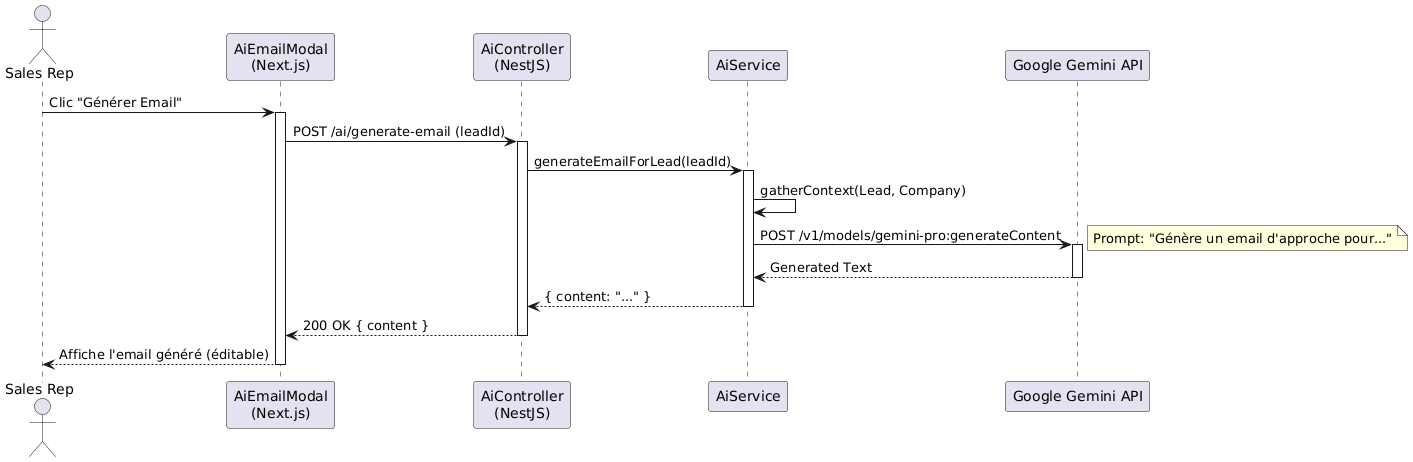
\includegraphics[width=\textwidth,height=0.82\textheight,keepaspectratio]{images/dsc_gemini_email.png}
    \caption{Diagramme de séquence de conception \og~Générer Email avec Gemini~\fg{}}
    \label{fig:dsc_gemini}
\end{figure}

\subsection{Diagramme de classes participantes (DCP)}

Le diagramme de classes participantes (DCP) fait le lien entre les cas d’utilisation, l'interface utilisateur et les diagrammes de conception logicielle. Il modélise les classes de dialogue (les composants Next.js), les classes de contrôle (les Services et Contrôleurs NestJS) et les entités (les Modèles Prisma).

\subsubsection{DCP du cas d'utilisation \og~Gérer les Leads~\fg{}}

Dans ce diagramme, nous observons l’interaction des composants d'interface (\texttt{LeadsTable}, \texttt{LeadDetailsModal}) avec le contrôleur \texttt{LeadsController}. Ce dernier interroge et modifie les informations en faisant appel au \texttt{LeadsService}, qui s'occupe de persister ou de récupérer les entités \texttt{Lead}, \texttt{Contact} et \texttt{Company} dans la base de données.

\begin{figure}[H]
    \centering
    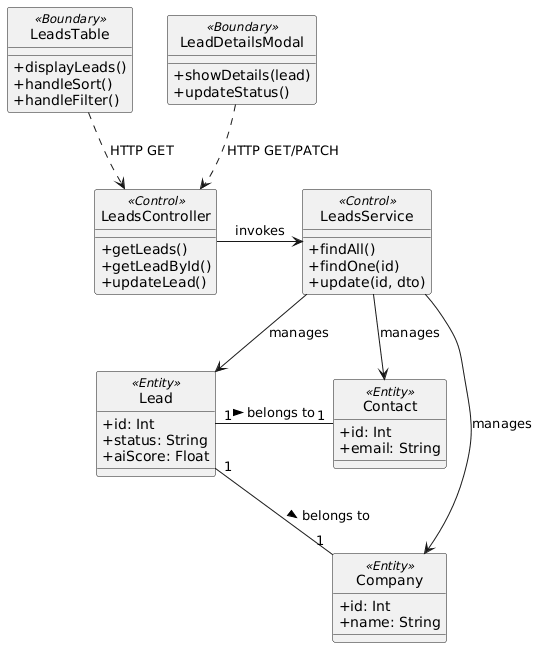
\includegraphics[width=\textwidth,height=0.82\textheight,keepaspectratio]{images/dcp_gerer_leads.png}
    \caption{DCP du cas d'utilisation \og~Gérer les Leads~\fg{}}
    \label{fig:dcp_leads}
\end{figure}

\subsubsection{DCP du cas d'utilisation \og~Importer Données CSV~\fg{}}

Ce diagramme illustre la communication entre le composant d'importation \texttt{CSVImportWizard} et les contrôleurs backend correspondants. Le \texttt{ImportService} réceptionne et analyse le fichier, manipule les \texttt{CreateContactDto} ou \texttt{CreateLeadDto}, effectue la validation, et insère les entités résultantes dans la base pour traiter les données en masse.

\begin{figure}[H]
    \centering
    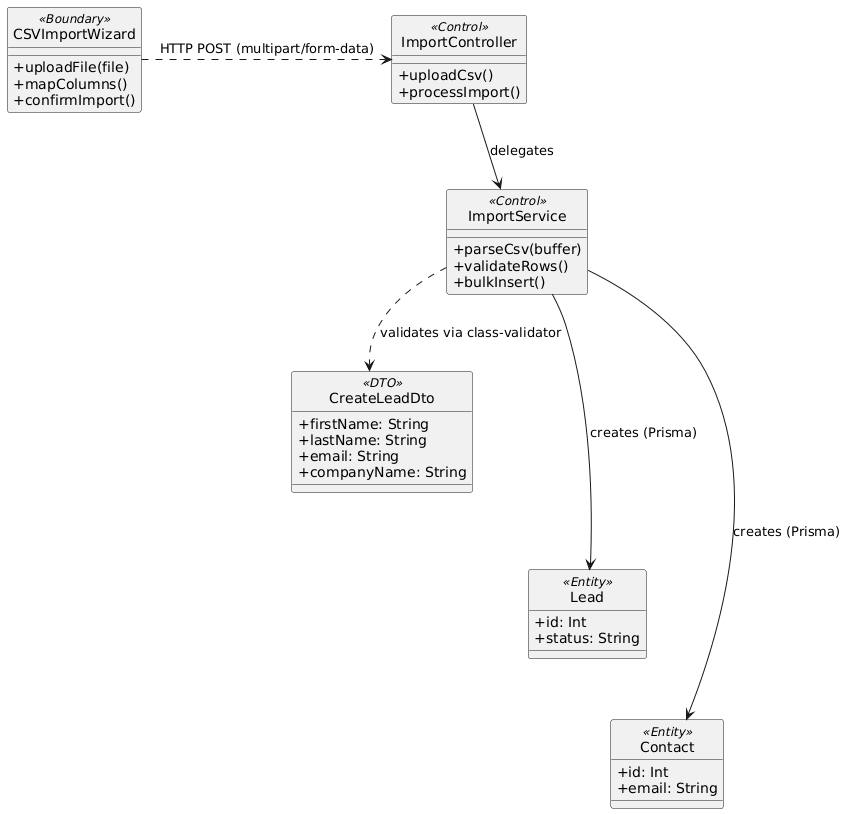
\includegraphics[width=\textwidth,height=0.82\textheight,keepaspectratio]{images/dcp_import_csv.png}
    \caption{DCP du cas d'utilisation \og~Importer Données CSV~\fg{}}
    \label{fig:dcp_import}
\end{figure}

\subsection{Diagramme de blocs internes}

Le diagramme de blocs internes offre une vue d'ensemble de la hiérarchie et de la distribution des responsabilités au sein des différents niveaux de notre système. Inspiré par les architectures en couches robustes, ce modèle illustre l'intégration entre la couche de présentation (les composants d'interface), la logique applicative (les contrôleurs et les services) et la logique métier (les entités de la base de données). Il met en évidence la fluidité de la communication verticale, depuis l'interaction de l'utilisateur jusqu'à la persistance des données.

\begin{figure}[H]
    \centering
    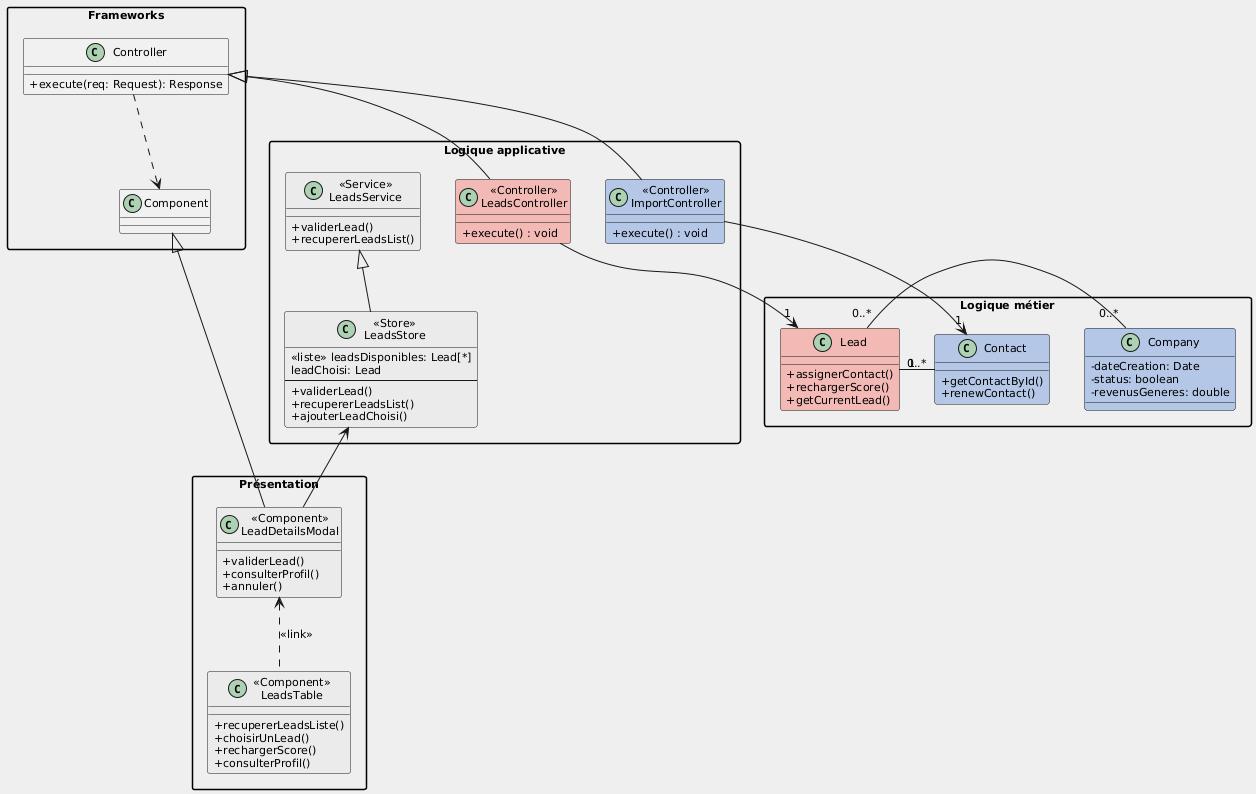
\includegraphics[width=\textwidth,height=0.82\textheight,keepaspectratio]{images/diagramme_blocs_internes.png}
    \caption{Diagramme de blocs internes du système}
    \label{fig:diagramme_blocs_internes}
\end{figure}

%──────────────────────────────────────────────────────
\section*{Conclusion}
\addcontentsline{toc}{section}{Conclusion}
%──────────────────────────────────────────────────────

Ce chapitre a permis de passer de la vision fonctionnelle abstraite à une perspective technique et conceptuelle précise. L'architecture orientée services adoptée, qui combine Next.js, NestJS et FastAPI, fournit une séparation nette des responsabilités, modélisée selon l'approche 3-tiers. L'utilisation de patrons de conception standards de l'industrie (MVC, DAO, DTO) garantit une base de code maintenable, sécurisée et pérenne. Par l'élaboration des diagrammes de classes (structure statique) et de séquences (comportement dynamique), nous avons pu dresser une cartographie complète du fonctionnement interne du logiciel. L'application est dorénavant prête pour la phase d'implémentation, qui sera abordée dans le chapitre suivant.
